%/*% pdflatex -file-line-error -interaction nonstopmode %

\documentclass{article}
\usepackage{graphicx}
\usepackage{amsmath}
\usepackage{amsfonts}
\usepackage{bookmark}
\usepackage{booktabs}
\usepackage{exercises}
\graphicspath{ {./images/2.8} }
\usepackage{indentfirst}
\usepackage{amsthm}
\usepackage{yhmath}
\usepackage{placeins}
\newcommand*{\oldneg}{\mathord{\sim}}
\newcommand\showdiv[1]{\overline{\smash{)}#1}}
\newcommand\Mydiv[1]{%
\smash{\raise.3ex\hbox{$\big)$}}\mkern-8mu
        \overline{\enspace\strut#1}}
\setlength{\tabcolsep}{5pt}
\theoremstyle{definition}
\newtheorem{definition}{Definition}

\setlength{\parindent}{.5in}
\setlength{\parskip}{12pt}
\renewcommand{\arraystretch}{1}

\title{2.8 Answers}
\begin{document}
\maketitle

\section*{1}


A local maximum or local minimum of a polynomial function occurs at a turning point of the function's graph.

\section*{2}


A local maximum of a function is defined to be a point of a function such that it is greater than all nearby points. This differs from the maximum value in the function in that 
the maximum of the function must be greater than $all$ other points in the function, not just nearby points.

\section*{12}


We know that one zero of this function is $4$, because $x-4$ is a factor of $h(x)$. The other factor, $2x^2-2x+1$, is a quadratic function, and has two imaginary solutions, as 
\[ b^2-4ac=(-2)^2-4(2)(1)=-4<0 \] meaning these other zeros are not graphable in this situation. Thus, we only need to graph the zero $x=4$. Also, we know that, because this is a 
polynomial of degree three (odd) and having a positive leading coefficient, $f(x)\rightarrow +\infty$ as $x\rightarrow +\infty$, and $f(x)\rightarrow -\infty$ as $x\rightarrow -\infty$:
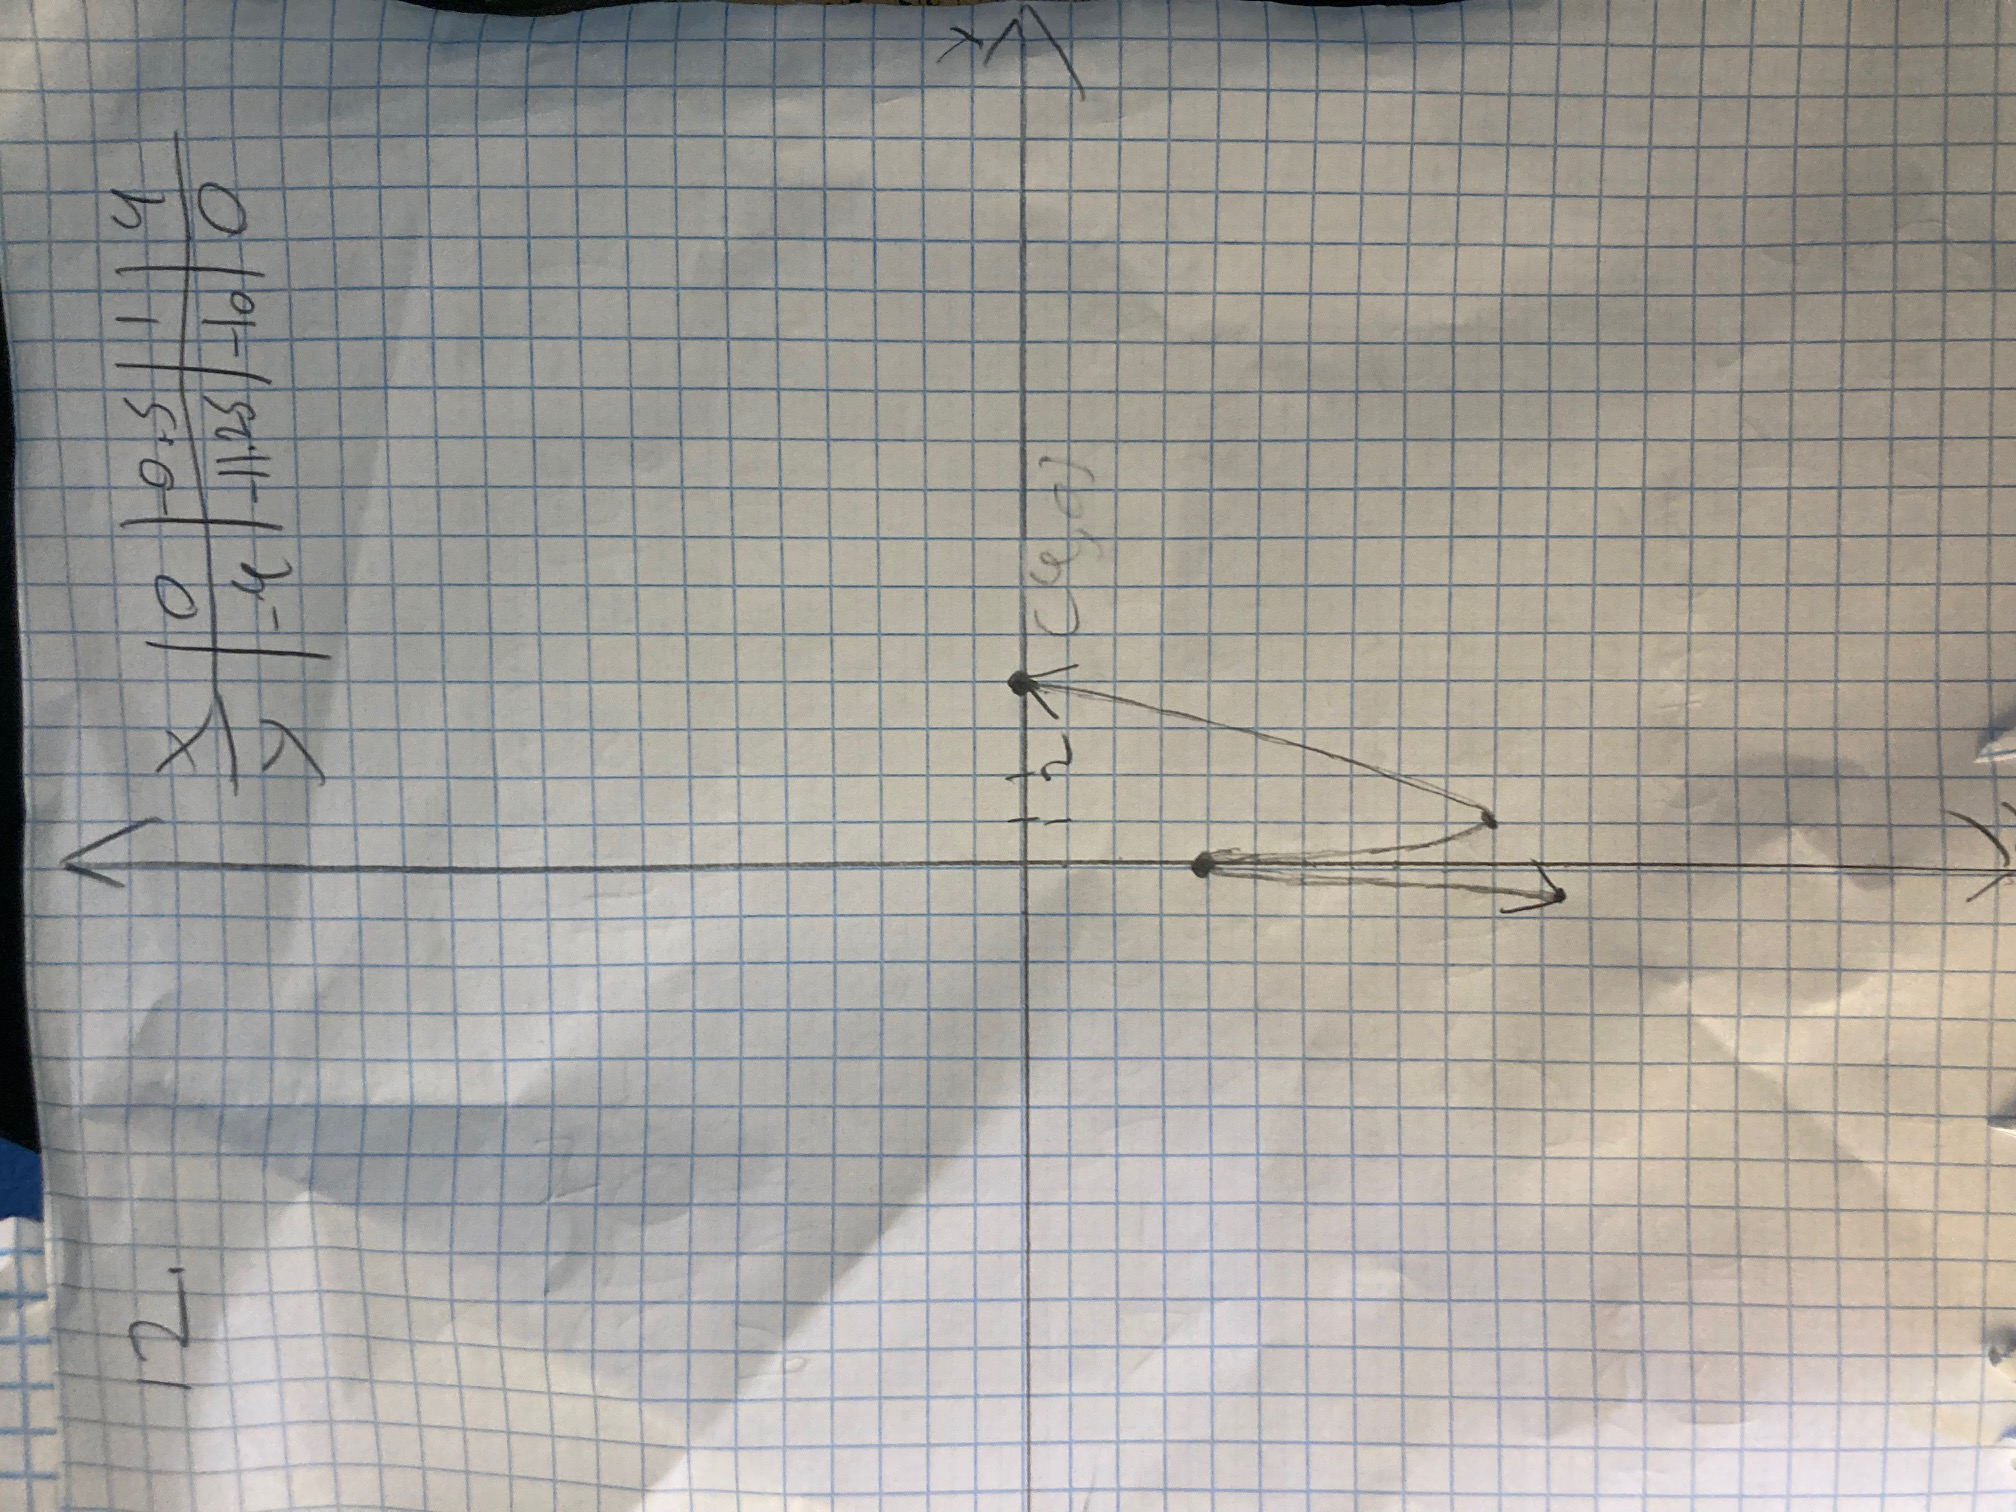
\includegraphics[width = 4in, height = 4in, angle = -90]{12}


\section*{13} 


The error here is that the $x$-intercepts were graphed incorrect. Instead of graphing the $x$-intercepts of $-1$ and $2$, the actual $x$-intercepts are $-2$ and $1$. 

\section*{14}

In this example, while the $x$-intercepts are graphed correctly, the end behavior is incorrect. In particular, we are dealing with a quartic polynomial with a positive leading 
coefficient, meaning $f(x)\rightarrow +\infty$ in both directions. However, in the graph, $f(x)\rightarrow -\infty$ as $x\rightarrow -\infty$. This can be corrected by 
simply drawing the arrow up instead of down.

\section*{20}


Local maxima estimates: $(-0.5,-0.5)$. Local minima estaimtes: $(-1.75,2),(0.5,-2)$. We know that a polynomial function of degree $n$ has at most $n-1$ turning points, 
meaning the least degree that this function can have is $n=3+1=4$. This fits with the known end-behavior of ths graph, as it corresponds to an even degree with a positive 
leading coefficient (and 4 is even).

\section*{21}


Using a graphing calculator, we can see that the answer is B.

\section*{29}

We can see that the local maximum is $(0.469,1.554)$, while the local minima are 
$(8.547,-1216.679),(-0.445,-1.493)$. 
Because we are considering a quartic polynomial, we know that is has at most 
$3$ turning points. Because we have already identified 3 turning points, we know that we have identified 
all the turning points of this function. In addition, we see that the $x$-intercepts are $(-0.765,0),(0,0),(0.821,0),$ and $(11.373,0)$. Because we are dealing with a quartic polynomial, 
we know by the fundemental theorem of algebra that this function has exactly $n=4$ zeros. Because we have found 4 real zeros, we know that we have found all the $x$-intercepts 
of this function.

\section*{30}


Using a graphing calculator, we can see that the answer is D.

\section*{31}


In a quadratic function, the parabola contains the vertex, and after that, the function continuously increases or decreases, depending on the value of $a$. This means that 
the vertex, which is also the maximum or minimum of the function, is the only maximum or minimum, and therefore there is no need to say that the vertex is a local 
maxima or minima, as there is only one.

\section*{32}


It is a fact that, if a polynomial has $n$ distinct real zeros, then it's graph has $exactly$ n-1 turning points. By Descartes' rule of signs, a cubic function either has 
$3$ or $1$ real zeros (which can be seen from Problem 51 in 2.7). This means that, if the function has $1$ real zero, it also would have 
$0$ turning points. However, it could have $2$ turning points if it had $3$ real zeros. Thus, a cubic function $sometimes$ has no turning points.

\section*{38}


We know that, for odd-degree polynomial functions, $f(x)\rightarrow +\infty$ as $x\rightarrow +\infty$ 
or $x\rightarrow -\infty$, and $f(x)\rightarrow -\infty$ in the oppose direction. Thus, the domain is 
$-\infty <x<+\infty$, while the range is $-\infty <x<+\infty$. With even degreed functions, however, 
we know that either $f(x)\rightarrow +\infty$ or $f(x)\rightarrow -\infty$ in both directions. In 
the first case, the minimum of the entire function is the lowest $y$ value of the local minima, 
call it $m$. Then, the domain of the function is $-\infty <x<+\infty$ and the range is $m\le x<+\infty$. 
On the other hand, if the leading coefficient is negative, then the maximum of the entire function is 
the highet $y$ value of the local maxima, call it $m$. Then, the domain of the function is 
$-\infty <x<+\infty$ while the range is $-\infty <x\le m$.

\section*{40}


We are trying to find the maximum volume of the box made of a cardboard that is 30 centimeters by 40 centimeters. If we follow the method described in Example 3, we know 
that:
\[ V=(40-2x)(30-2x)x \]
\[ V=(40-2x)(30x-2x^2) \]
\[ V=4x^3-140x^2+1200x \]
Which has the following graph:
\FloatBarrier
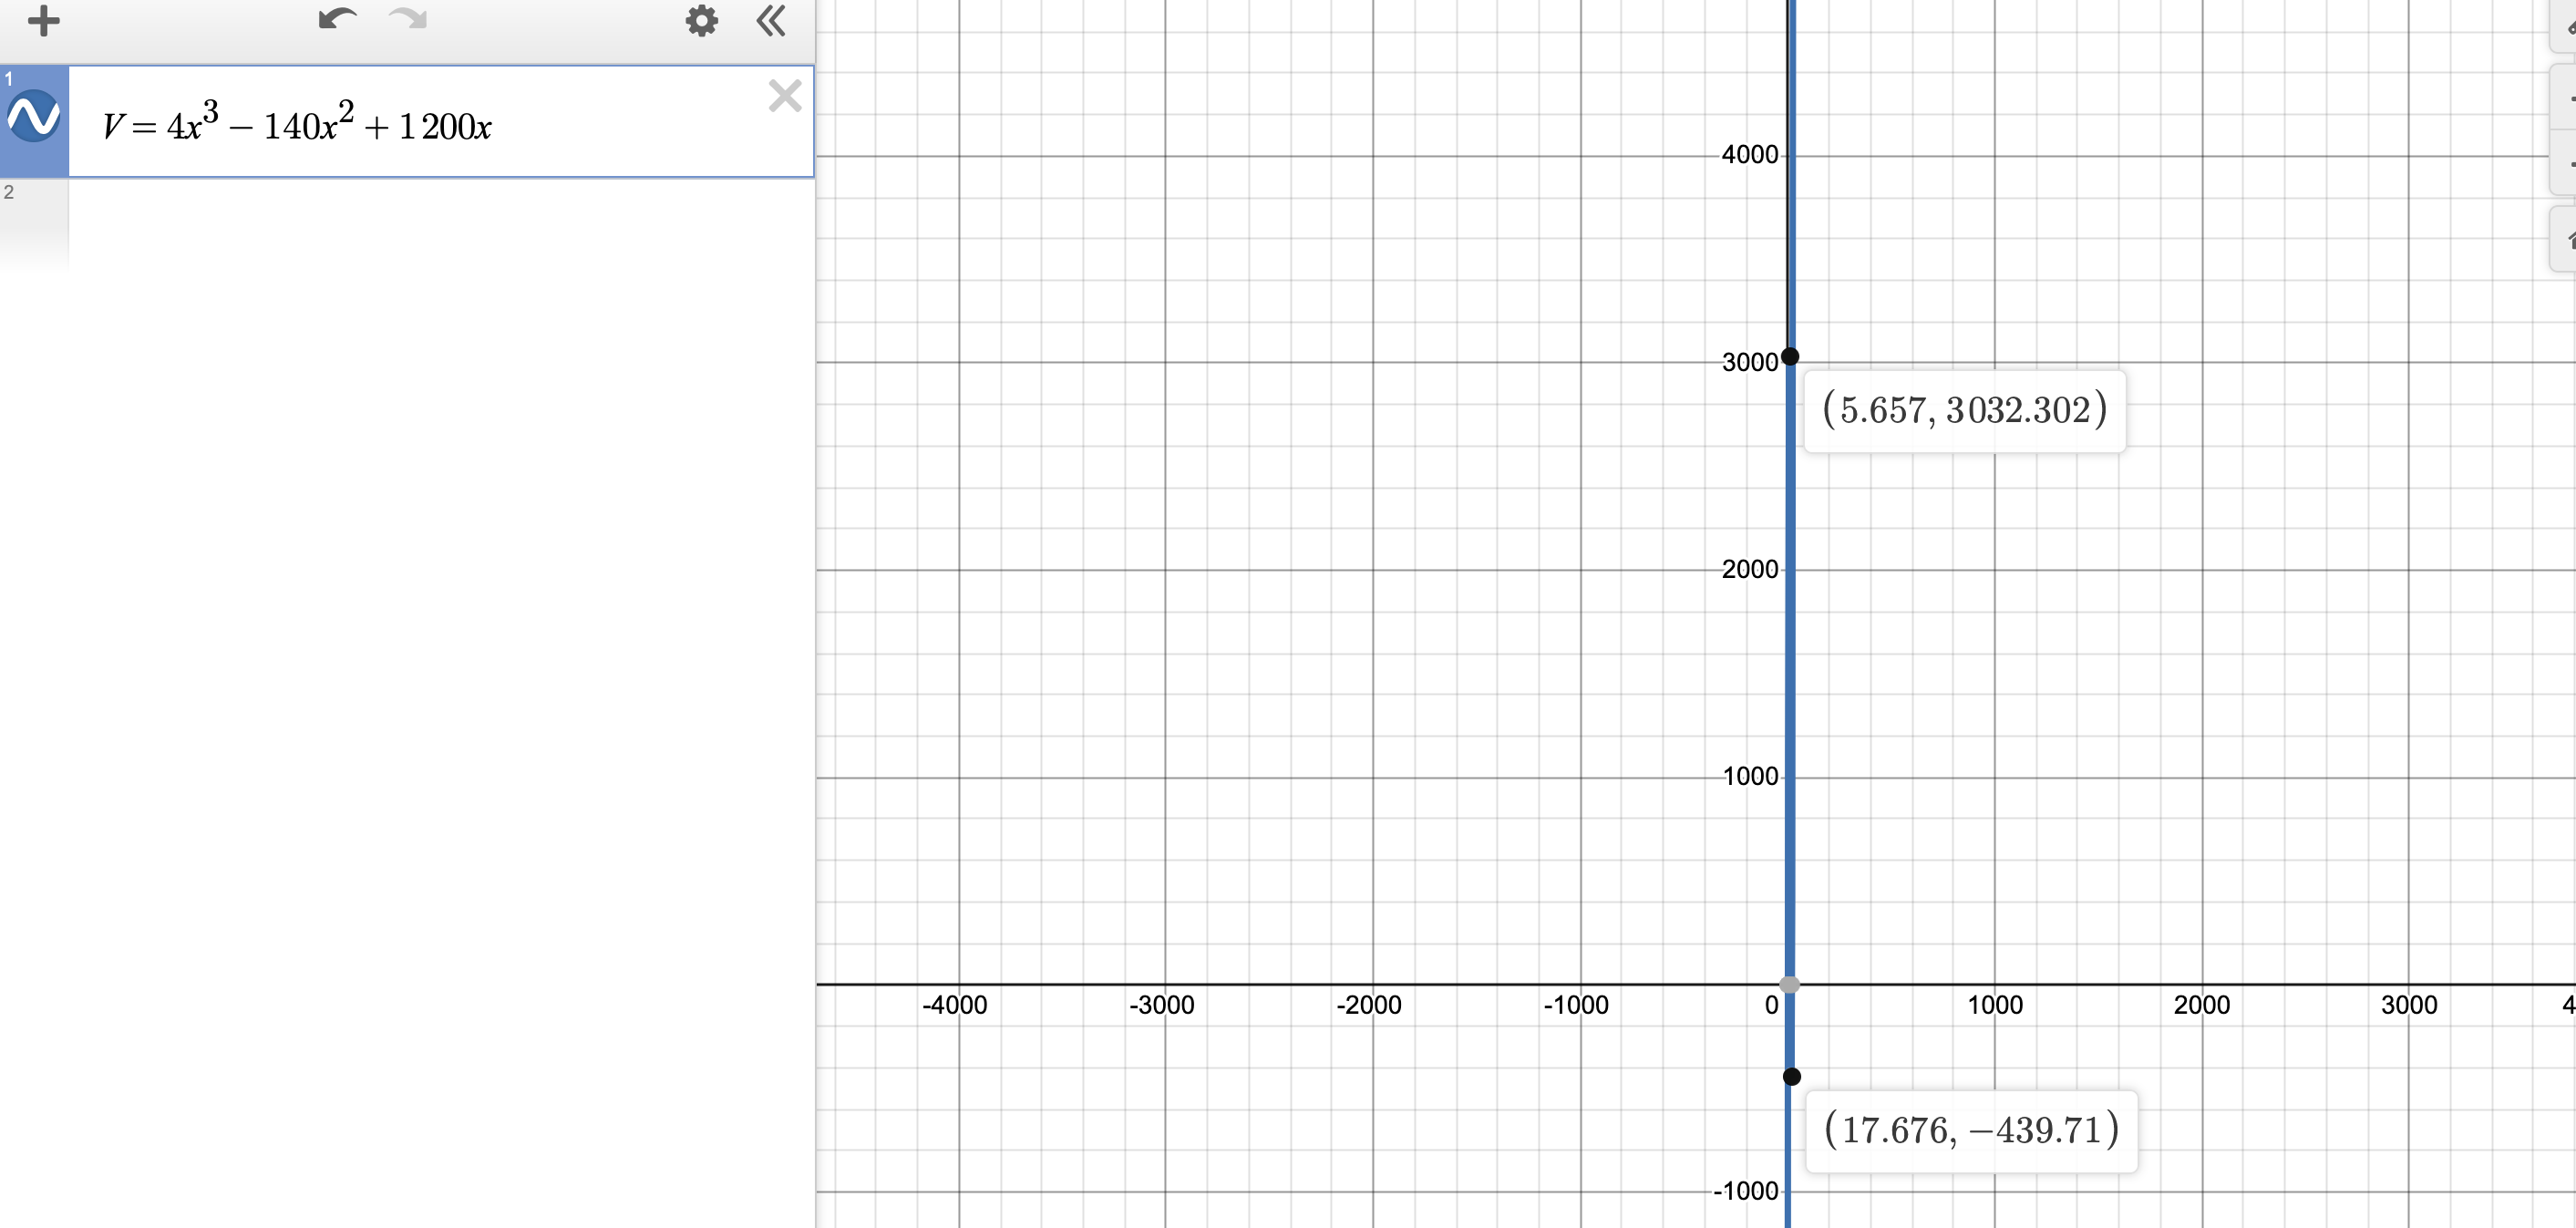
\includegraphics[width = 4in, height = 4in]{40}
\FloatBarrier
Now, we must consider only the range $0<x<15$, as $x$, the height, obviously cannot be negative; if it was $\ge 15$, then one of the dimensions would be $30-2(x)<0$, 
which is also impossible. From the graph, we can see that a maximum value is $5.657,3032.302$ and a minimum value is $17.676,-439.71$. Because we are considering a cubic function, it 
has at most $2$ turning points, meaning $5.657,3032.302$ is the only local maximum. Because it is in the desired domain, we know that the maximum volume is $3032.302$ cubic cm, 
while the dimensions 
are $5.657$ cm high by $40-2(5.657)=28.686$ cm by $18.686$ cm.

\section*{42}


(a): Substituting $600$, we get:
\[ 600=\pi r^2+\pi rl \]
Solving for $l$, we get:
\[ 600=\pi r^2+\pi rl \]
\[ -\pi rl=\pi r^2-600 \]
\[ l=-r+\frac{600}{\pi r} \]
(b): We know that: \[ V=\frac{1}{2}\pi r^2l \] We can substitute the result that we got from (a) in this equation for $l$, thus yielding:
\[ V=\frac{1}{2}\pi r^2(-r+\frac{600}{\pi r}) \]
\[ V=\frac{1}{2}(-r^3\pi +600r) \]
(c): The equation from part (b) has the following graph:
\FloatBarrier
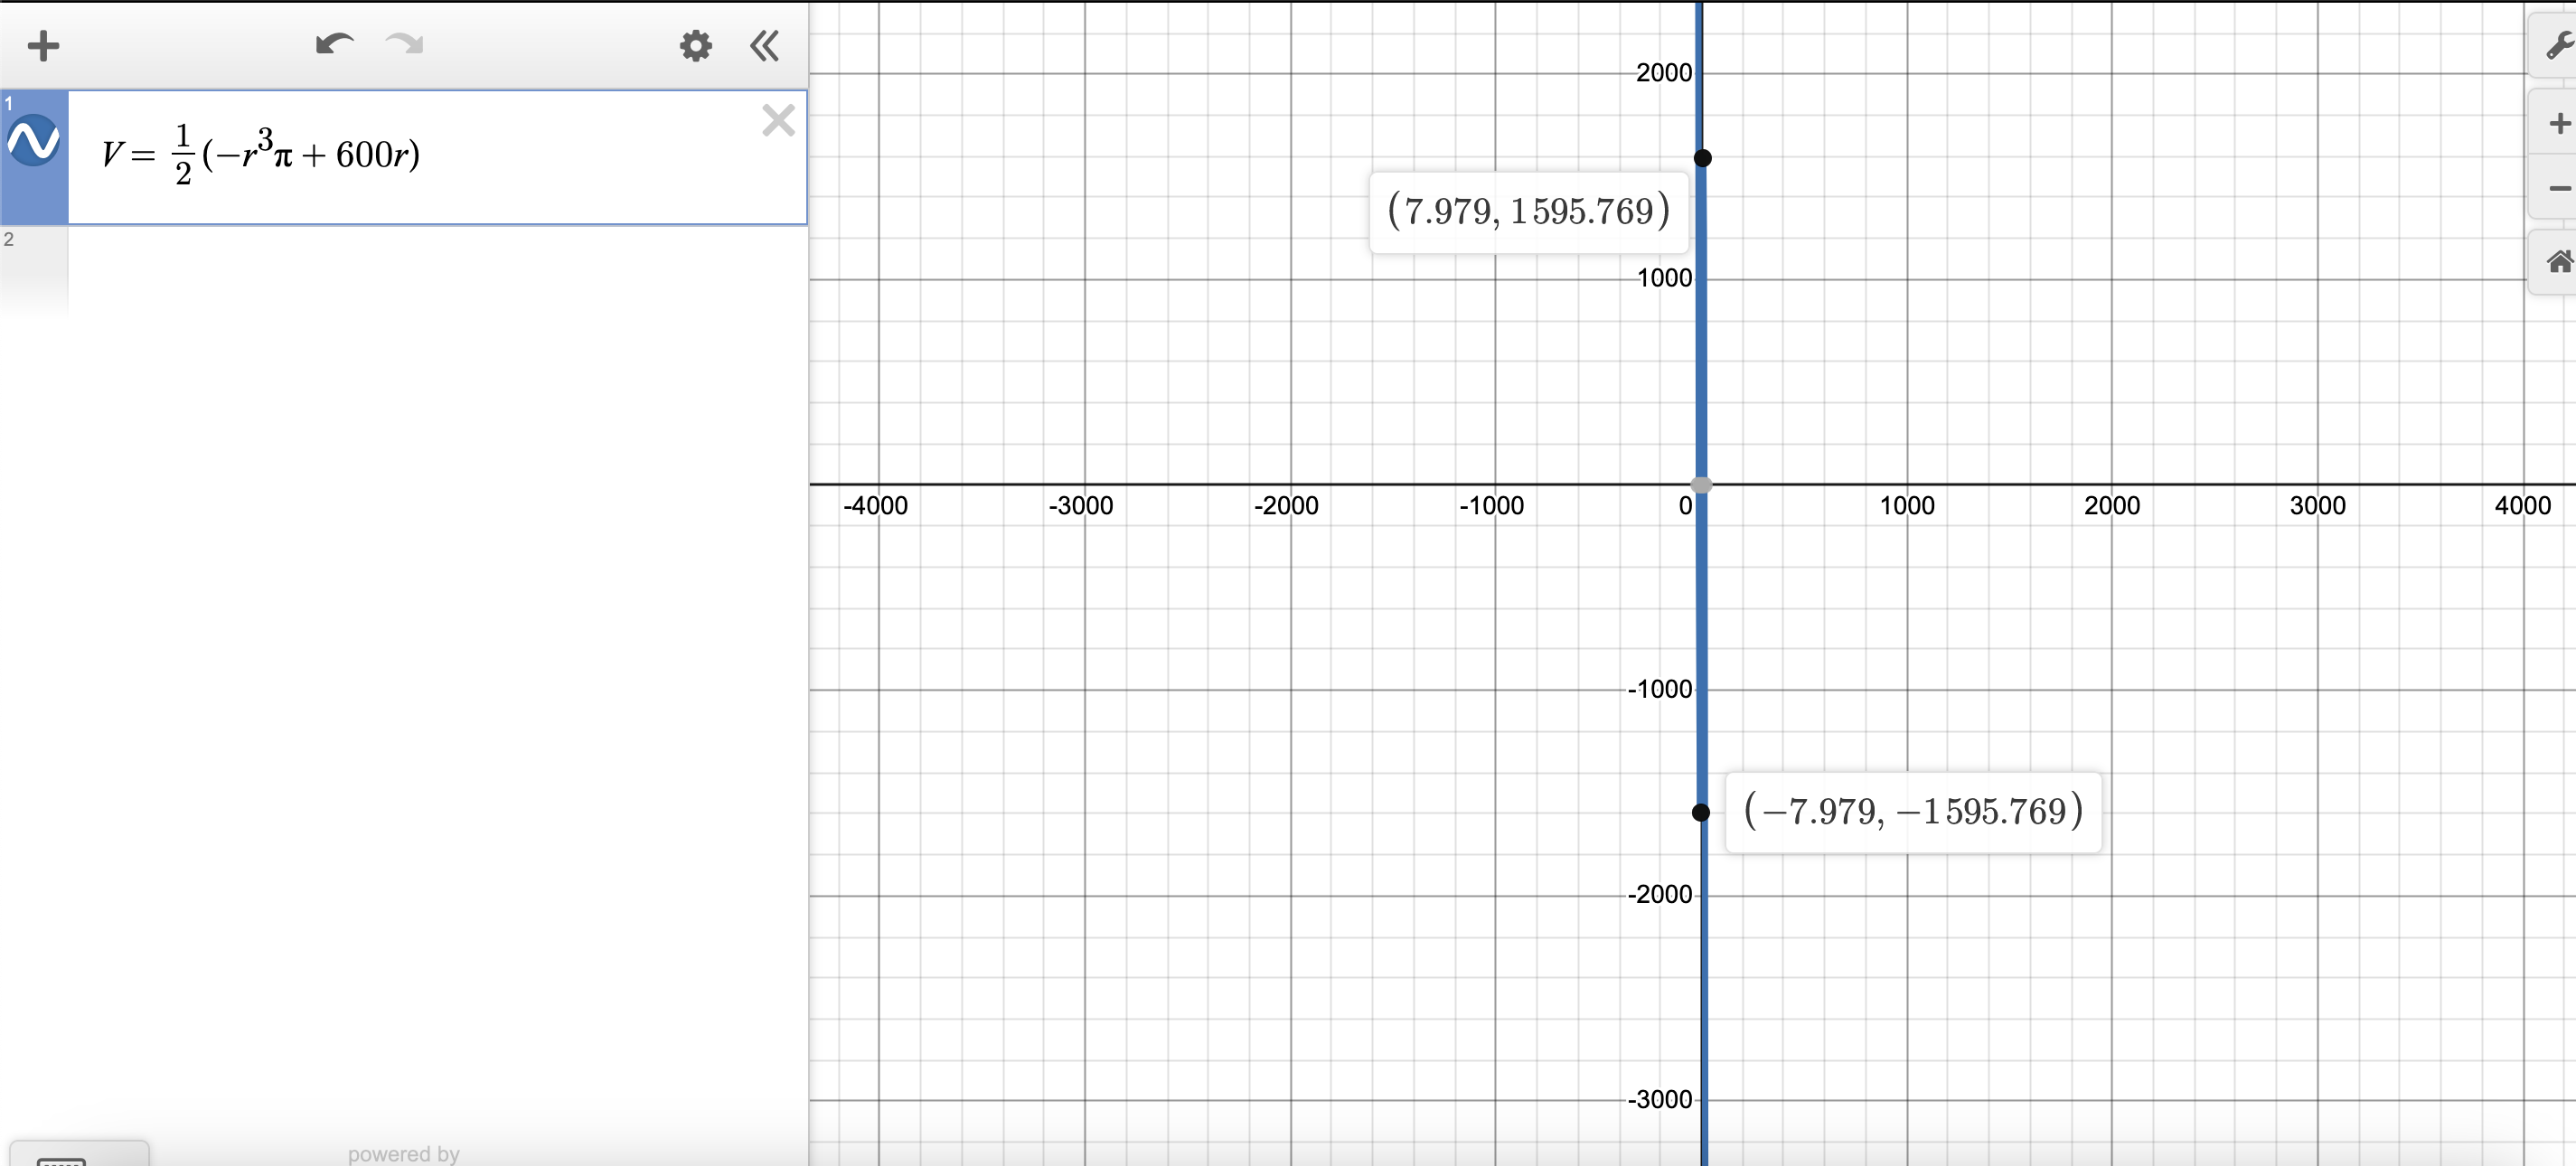
\includegraphics[width = 4in, height = 4in]{42}
\FloatBarrier
We can see that a local maximum is $7.979,1595.769$, and a local minimum is $(-7.979,-1595.769)$. Because we are dealing with a cubic polynomial, it has at most $2$ turning points. 
Because we have found 2 turning points, we have therefore found all of it's turning points. Thus, $7.979,1595.769$ is the local maximum in the range $0<x<15$.
Thus, a radius of $r=7.979$ and a length of 
\[ -7.979+\frac{600}{\pi\times 7.979}\approx 15.957 \] produces a maximum volume of about 
\[ \frac{1}{2}\pi (7.979)^2 15.957\approx 1595.762 \] cubic feet.

\section*{44}


First, we can see from the picture that we can form a right triangle with the hypotenuse as $2\times 8=16$, one of the legs as $h$, and the other as $d$, the diameter of the cylinder. 
By the Pythagorean theorem, we have:
\[ d^2+h^2=16^2 \]
\[ d^2=256-h^2 \]
\[ \textrm{(1) } d=\sqrt{256-h^2} \]
We are asked to find the volume of $h$ that maximizes the volume of the inscribed cylinder. The cylinder has a volume of:
\[ V=\pi r^2h \] where \[ r=\frac{d}{2} \] meaning
\[ V=\pi (\frac{d}{2})^2h=\pi\frac{d^2h}{4}=\frac{1}{4}\pi d^2h \] We can substitute the value we recieved for $d$ in equation (1) to write the volume equation in terms of $h$:
\[ V=\frac{1}{4}\pi (\sqrt{256-h^2})^2h=\frac{1}{4}\pi (256-h^2)h=\frac{1}{4}(256h\pi -h^3\pi) \]
The graph of the above function is:
\FloatBarrier
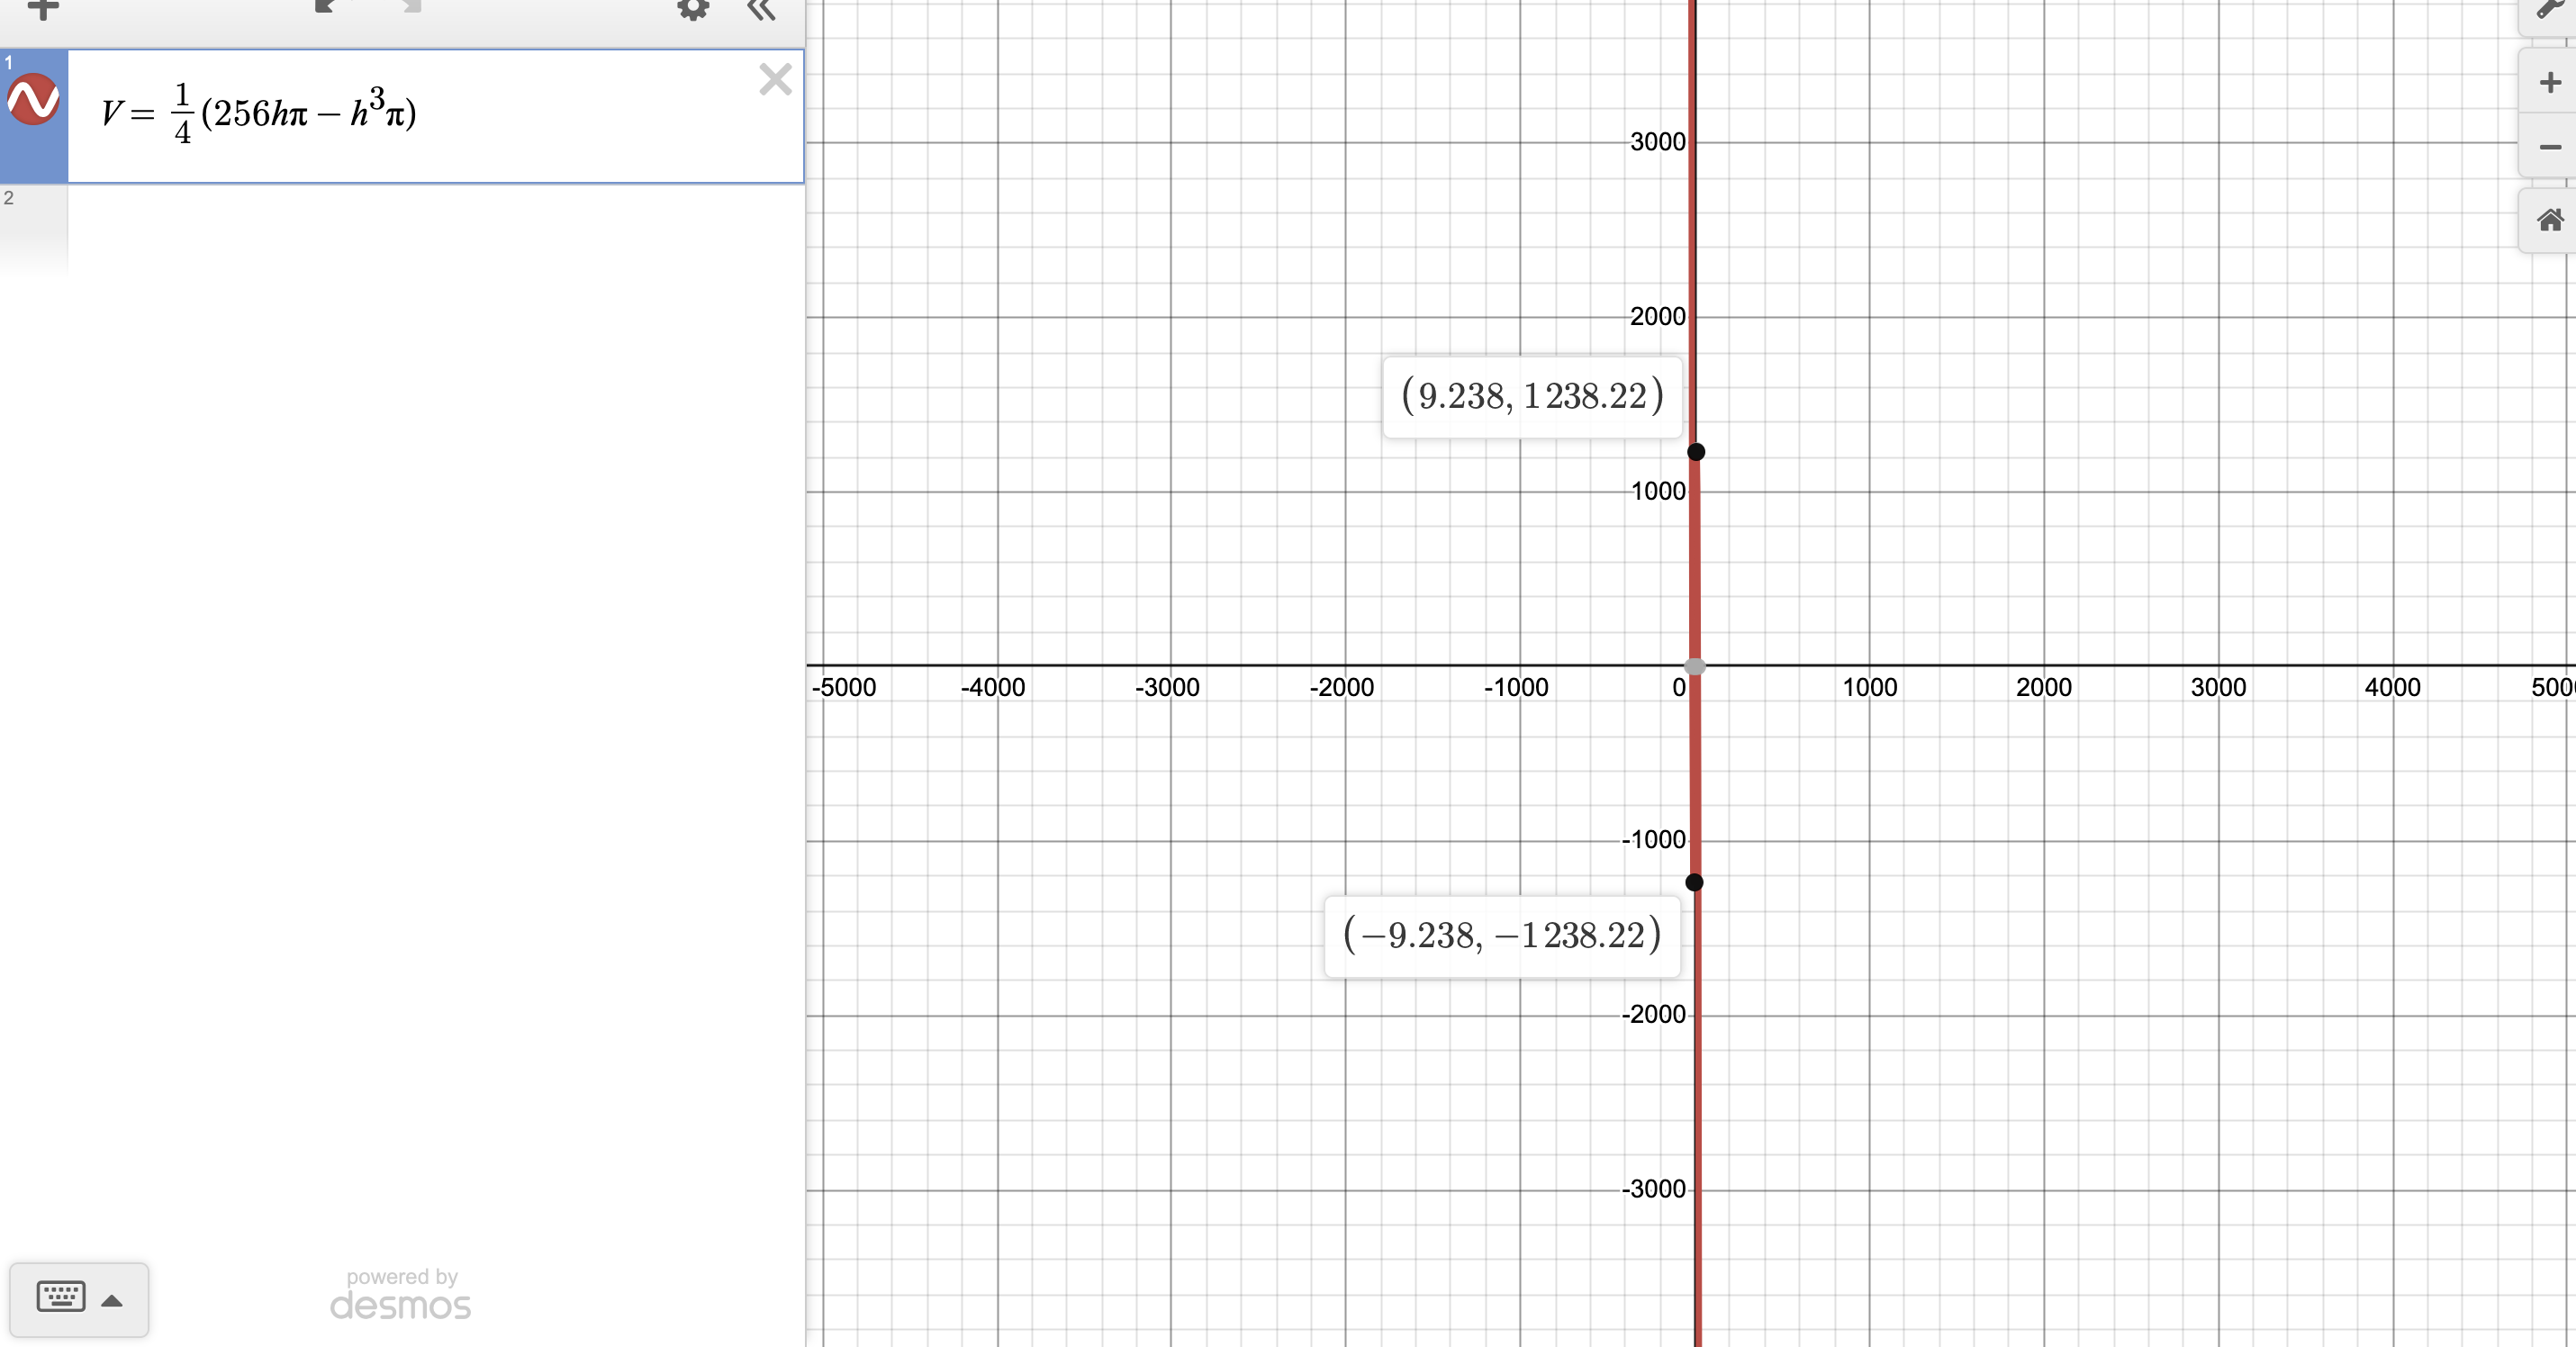
\includegraphics[width = 4in, height = 4in]{44}
\FloatBarrier
We can see that the graph has one local maximum: (9.238,1238.22), and one local minimum: (-9.238,-1238.22). Because this is a cubic function, it has at most $2$ turning points. Because we have 
found two turning points, we have found all the turning points of the function. Also, this is a polynomial function of degree 3 (odd) with a negative leading coefficient, 
meaning $f(x)\rightarrow -\infty$ 
as $x\rightarrow +\infty$ and $f(x)\rightarrow +\infty$ as $x\rightarrow -\infty$. We know that all the answers where $h\le 0$ are impossible, as measurements cannot be negative here. Thus, we can 
conclude that the one local maximum, (9.238,1238.22), is the highest positive measurement. Therefore, the maximum volume is $1238.22$ cubic units, having a height of $9.238$.




\end{document}

